\documentclass[12pt]{report}
\usepackage[a4paper]{geometry}
\usepackage[T1]{fontenc}
\usepackage{amsmath}
\usepackage{amssymb}
\usepackage{fancyhdr}
\usepackage{float}
\usepackage{graphicx}
\usepackage[table,xcdraw]{xcolor}
\usepackage{hyperref}
\usepackage{appendix}
\usepackage[printonlyused]{acronym}
\usepackage{multirow}
\usepackage{url}
\usepackage{subfig}
\usepackage{listings}
\usepackage{siunitx}
\lstdefinelanguage{NetLogo}{
    basicstyle=\small,
    breaklines=true,
    breakatwhitespace=true,
    alsoletter={-,?,.},
    morekeywords=[1]{to, to-report, end, __includes, breed, globals, pseudopodia-own, foods-own, tubes-own, searchers-own, patches-own},
    keywordstyle=[1]\color[rgb]{0.0, 0.66, 0.42},
    morekeywords=[2]{ask, let, set, if, report, ifelse, clear-all, reset-ticks, die, create-link-with, face, fd, setxy, pen-down, hatch},
    keywordstyle=[2]\color{blue},
    morekeywords=[3]{patch, patches, xcor, ycor, of, random-float, with, any?, one-of, turtle-set, turtles-on, patch-ahead, pcolor, ranodm, not, can-move?, length, in-radius, item, neighbors, abs, pxcor, max-pxcor, pycor, max-pycor, size, myself, shabe, color, other, link-with, length, replace-item, map, list, and, or, not, n-of, min-pxcor, min-pycor, label-color, myself, sqrt, max, distance, insert-item, shape, hidden?, label},
    keywordstyle=[3]\color[rgb]{0.74, 0.2, 0.64},
    morekeywords=[4]{nobody},
    keywordstyle=[4]\color[rgb]{0.86, 0.08, 0.24},
    comment=[l]{\;},
    commentstyle=\color[rgb]{0.75,0.75,0.75},
    string=[d]{"},
    stringstyle=\color{orange},
    morekeywords=[5]{1, 2, 3, 4, 5, 6, 7, 8, 9, 0, true, false},
    keywordstyle=[5]{\color{orange}},
}
\lstdefinestyle{jsonstyle}{
  basicstyle=\ttfamily\small,
  breaklines=true,
  breakatwhitespace=false,
  columns=flexible,
  frame=single,
  language={}
}
\lstdefinestyle{pythonstyle}{
    language=Python,
    basicstyle=\ttfamily\small,
    breaklines=true,
    breakatwhitespace=false,
    numbers=left,
    numberstyle=\tiny,
    keywordstyle=\color{blue},
    commentstyle=\color{gray},
    stringstyle=\color{orange},
    showstringspaces=false,
    frame=single
}

\usepackage[acronym]{glossaries}
\usepackage{afterpage} \newcommand\blankpage{%
\null \thispagestyle{empty}%
  \addtocounter{page}{-1}%
    \newpage}
\usepackage{listings} \lstset{numbers=left, numberstyle=\tiny, numbersep=5pt} \lstset{language=Matlab}
\sloppy
\graphicspath{{images/}}

\setlength{\textwidth}{15 true cm}
\setlength{\textheight}{22 true cm}
\setlength{\headheight}{15pt}
\oddsidemargin  0.5 cm
\evensidemargin 0.5 cm
\topmargin      -1.0 cm

\usepackage{url}
\urlstyle{tt}
\urldef{\test}{\url{http://de.wikipedia.org/wiki/Hilfe:TeX}}

%\newcommand{\tanh}{\operatorname{tanh}}

\widowpenalty=10000
\clubpenalty=10000
\begin{document}

\begin{titlepage}
\begin{center}

    {\LARGE FirstName LastName\\}
    \vspace{5mm}
    \rule{\textwidth}{1pt}
%	\vspace*{3mm}
	{ \LARGE Title  \\
	\vspace*{3mm}Subtitle}
	\vspace*{3mm}
\rule{\textwidth}{1pt}

    \vspace{15mm}
	{\LARGE \sc MASTER THESIS} \\
    \vspace{8mm}
	\normalsize{submitted in fulfilment of the requirements for the degree of}\\
	\vspace{8mm}
	\Large{Diplom-Ingenieurin}\\
	\vspace{8mm}
	\normalsize{Programme: Master’s programme Information and Communications Engineering}\\	\vspace{2mm}
	\normalsize{Branch of study: Autonomous Systems and Robotics}\\
	\vspace{2mm}
     \vspace{8mm}%15
	\Large{Alpen-Adria-Universit\"at Klagenfurt}\\
    \vspace{4mm}
    
\includegraphics[width=0.35\textwidth]{images/uniklulogo.png}

  \vspace{0.5 mm}%15
  -------------------------------------- \\
\end{center}

    \vspace{1mm}
    \enlargethispage{1cm}

\begin{tabular}{ l l }

\textbf{Evaluator}\\
Univ.--Prof. Dipl.--Ing. Dr. techn. Wilfried Elmenreich \\
Alpen-Adria-Universit\"at Klagenfurt \\
Institut f{\"u}r Vernetzte und Eingebettete Systeme \\

\end{tabular}


\vspace{10mm}
\raggedleft{Klagenfurt, \today}\\    

\end{titlepage}

\afterpage{\blankpage}
	
	
\pagestyle{fancy}
\pagenumbering{roman}
\rfoot{\thepage}
\cfoot{}
\include{stmt}
{\Large
\noindent
{\bf Affidavit}} \\
\vspace*{0.3 cm}

\noindent
I hereby declare in lieu of an oath that
\begin{itemize}
    \item[-] the submitted academic paper is entirely my own work and that no auxiliary materials have been used other than those indicated,
    \item[-] I have fully disclosed all assistance received from third parties during the process of writing the thesis, including any significant advice from supervisors,
    \item[-] any contents taken from the works of third parties or my own works that have been included either literally or in spirit have been appropriately marked and the respective source of the information has been clearly identified with precise bibliographical references (e.g. in footnotes),
    \item[-] to date, I have not submitted this paper to an examining authority either in Austria or abroad and that
    \item[-] when passing on copies of the academic thesis (e.g. in bound, printed or digital form), I will ensure that each copy is fully consistent with the submitted digital version.
\end{itemize}

\noindent
I am aware that a declaration contrary to the facts will have legal consequences.\\\\\\\\

\noindent
\begin{table}[H]
\centering{
\begin{tabular}{ll}
FirstName LastName m.p.\qquad \qquad \qquad & \qquad \qquad Klagenfurt, \today
\end{tabular}
}
\end{table}
{\Large
\noindent
{\bf Abstract}} \\
\vspace*{0.3 cm}

\noindent
Lorem ipsum dolor sit amet, consetetur sadipscing elitr, sed diam nonumy eirmod tempor invidunt ut labore et dolore magna aliquyam erat, sed diam voluptua. At vero eos et accusam et justo duo dolores et ea rebum. Stet clita kasd gubergren, no sea takimata sanctus est Lorem ipsum dolor sit amet. Lorem ipsum dolor sit amet, consetetur sadipscing elitr, sed diam nonumy eirmod tempor invidunt ut labore et dolore magna aliquyam erat, sed diam voluptua. At vero eos et accusam et justo duo dolores et ea rebum. Stet clita kasd gubergren, no sea takimata sanctus est Lorem ipsum dolor sit amet. Lorem ipsum dolor sit amet, consetetur sadipscing elitr, sed diam nonumy eirmod tempor invidunt ut labore et dolore magna aliquyam erat, sed diam voluptua. At vero eos et accusam et justo duo dolores et ea rebum. Stet clita kasd gubergren, no sea takimata sanctus est Lorem ipsum dolor sit amet. \\\\Duis autem vel eum iriure dolor in hendrerit in vulputate velit esse molestie consequat, vel illum dolore eu feugiat nulla facilisis at vero eros et accumsan et iusto odio dignissim qui blandit praesent luptatum zzril delenit augue duis dolore te feugait nulla facilisi. Lorem ipsum dolor sit amet, consectetuer adipiscing elit, sed diam nonummy nibh euismod tincidunt ut laoreet dolore magna aliquam erat volutpat.\\\\Ut wisi enim ad minim veniam, quis nostrud exerci tation ullamcorper suscipit lobortis nisl ut aliquip ex ea commodo consequat. Duis autem vel eum iriure dolor in hendrerit in vulputate velit esse
{\Large
\noindent
{\bf Zusammenfassung}} \\
\vspace*{0.3 cm}

\noindent
Lorem ipsum dolor sit amet, consetetur sadipscing elitr, sed diam nonumy eirmod tempor invidunt ut labore et dolore magna aliquyam erat, sed diam voluptua. At vero eos et accusam et justo duo dolores et ea rebum. Stet clita kasd gubergren, no sea takimata sanctus est Lorem ipsum dolor sit amet. Lorem ipsum dolor sit amet, consetetur sadipscing elitr, sed diam nonumy eirmod tempor invidunt ut labore et dolore magna aliquyam erat, sed diam voluptua. At vero eos et accusam et justo duo dolores et ea rebum. Stet clita kasd gubergren, no sea takimata sanctus est Lorem ipsum dolor sit amet. Lorem ipsum dolor sit amet, consetetur sadipscing elitr, sed diam nonumy eirmod tempor invidunt ut labore et dolore magna aliquyam erat, sed diam voluptua. At vero eos et accusam et justo duo dolores et ea rebum. Stet clita kasd gubergren, no sea takimata sanctus est Lorem ipsum dolor sit amet.   \\\\Duis autem vel eum iriure dolor in hendrerit in vulputate velit esse molestie consequat, vel illum dolore eu feugiat nulla facilisis at vero eros et accumsan et iusto odio dignissim qui blandit praesent luptatum zzril delenit augue duis dolore te feugait nulla facilisi. Lorem ipsum dolor sit amet, consectetuer adipiscing elit, sed diam nonummy nibh euismod tincidunt ut laoreet dolore magna aliquam erat volutpat.\\\\Ut wisi enim ad minim veniam, quis nostrud exerci tation ullamcorper suscipit lobortis nisl ut aliquip ex ea commodo consequat. Duis autem vel eum iriure dolor in hendrerit in vulputate velit esse


\newpage
\vspace*{2.2 cm}
{\Large
\noindent
{\bf Acknowledgments}} \\
\vspace*{0.3 cm}

\noindent
Lorem ipsum dolor sit amet, consetetur sadipscing elitr, sed diam nonumy eirmod tempor invidunt ut labore et dolore magna aliquyam erat, sed diam voluptua. At vero eos et accusam et justo duo dolores et ea rebum. Stet clita kasd gubergren, no sea takimata sanctus est Lorem ipsum dolor sit amet. Lorem ipsum dolor sit amet, consetetur sadipscing elitr, sed diam nonumy eirmod tempor invidunt ut labore et dolore magna aliquyam erat, sed diam voluptua. At vero eos et accusam et justo duo dolores et ea rebum. Stet clita kasd gubergren, no sea takimata sanctus est Lorem ipsum dolor sit amet.


\newpage
\vspace*{2.2 cm}
\Large
\noindent
{\bf List of Acronyms} \\
\vspace*{0.7 cm}
\normalsize

\begin{acronym}
\acro{ACO}[ACO]{Ant Colony Optimization}
\acro{ADP}[ADP]{Adenosindiphosphat}
\acro{ATP}[ATP]{Adenosintriphosphat}
\acro{CYC}[CYC]{Cycle}
\acro{DLR}[DLR]{German Aerospace Center}
\acro{GUI}[GUI]{Graphical User Interface}
\acro{IDE}[IDE]{Integrated Development Environment}
\acro{IP}[IP]{Intersection Points}
\acro{KMG}[KMG]{Klagenfurt Mobil GmbH}
\acro{MAs}[MAs]{Metaheuristic algorithms}
\acro{NIOAs}[NIOAs]{Nature-Inspired Optimization Algorithms}
\acro{NED}[NED]{Network Description}
\acro{ÖBB}[ÖBB]{Österreichische Bundesbahnen}
\acro{pH}[pH]{Potential of Hydrogen}
\acro{PP}[PP]{Physarum Polycephalum}
\acro{SISMO}[SISMO]{SImulation of Slime MOld}
\acro{SMA}[SMA]{Slime Mold Algorithm}
\acro{SMT}[SMT]{Steiner´s Minimum Tree}
\acro{SOS}[SOS]{Self-Organizing Systems}
\acro{STW}[STW]{Stadtwerke}
\acro{SUMO}[SUMO]{Simulation of Urban Mobility}
\acro{WSNs}[WSNs]{Wireless Sensor Networks}
\end{acronym}

\afterpage{\blankpage} 

\newpage
\tableofcontents
\listoffigures
\listoftables
\clearpage


\pagestyle{plain}

\chapter{workplace}
\label{sec:workplace}
%This document is used to write text that does not have a proper location in the paper yet. I found that while writing I have a lot of issues understanding where to put certain text. This document is used to write that text and then move it to the right location in the paper.


\section{Design Science Research}

This thesis is based on the Design Science Research (DSR) methodology \cite{dresch2015design} and Computing as a discipline \cite{denning1989computing}. 

Computing as a discipline presents us with a framework for designing artefacts from an engineering point of view. It gives us four steps to solve a given problem:
\begin{enumerate}
    \item State requirements
    \item state specifications
    \item design and implement the system
    \item test the system
\end{enumerate}

For the requirements of this thesis we need to very specific as the thesis is working with two different requirements at the same time. The main research question is looking for the requirements of a comic book generating artefact thus the requirements of the research project should be linked to finding these artefact requirements. But that means that the requirements of the artefact itself can not be part of the requirements of the research project. The artefact requirements are part of the conclusion of the the thesis.


\subsection{Diverting from the DSR methodology}
In DSR you should start

---------------------------------------------------
\section{Retelling games}
Most people play games during their personal down time and do not really think about games outside of leisure context (REF). However there are also a lot of people that play games a lot and make it part of their lives. Looking at social media platforms like X, YouTube, Reddit, TikTok, etc. we can see that the sharing of gaming stories is a very big part of the internet. This sharing of stories can also be called retelling. Where people retell their personal stories about their gaming experiences. Retelling is not limited to games as the art of retelling is as old as humans and is a very big part of human culture(REF).

What is the essence of retelling? 

When talking about game retelling 


\subsection{Difference between retelling and storytelling}
\subsection{State of the art of retelling}
People share their gaming stories in many different ways. To have an holistic view of game retelling this section discussed the different forms of retelling video games.

Oldschool: talking
Podcast
YouTube
    Game play recording
        Podcasting
    Storytelling
    

An argument for Streaming.
For completion sake I want to mention streaming and unedited playthrough videos here as well. Streaming is a weird one when it comes to retelling as it is not a retelling of an experience, but a live experience.
    




\textit{Reteller is an agent that produces and narrates a sequence of events, for the benefit of either human players or spectators}\cite{Gallotta2024LLM}.

Retelling is one of the largest if not the largest cultural phenomenon out there. I would even say that the retelling is one of the reasons the internet has become as big as it is. All forms of social media became the behemoths they are because of people retelling their lives. Academics would not exist if we did not retell everything we do in the form of papers, books, lectures, etc. For this thesis- it is important to know what retelling is, how people interact with it, what the core aspects are of a retelling and which moments of the gameplay session are important and should be part of the retelling.

\chapter{Introduction}
\label{sec:intro}
\pagenumbering{arabic}
\section{Motivation and Objectives}

%Theatrical introduction
Storytelling has a rich history of development starting back as far as humanity can go back. From Neandertals 40.000 years ago making cave drawings in an attempt to share experience and knowledge and 5000 years ago the ancient Egyptians made Hieroglyphics to tell stories and record history. To now YouTubers sharing their experience and people on TikTok are recording and sharing everything they can think of. The medium of storytelling has been innovated time and time again, cave drawings, Hieroglyphics, oral, written texts, printing press, photo, film, and everything now in the digital age. But where are we going next? In a world that is ever-changing, super time hungry and where people are looking for more and more ways to consume and share stories. What is the next form of storytelling? What are new forms of storytelling we can use with new technology? As we are at the advent of a great generative artificial intelligence revolution we should look into the possibilities of AI. How can we use generative AI to create the next form of storytelling?

%Goal of the thesis
This thesis aims to look into the possible applicability of generative artificial intelligence and locally inferred large language models in combination with game retelling. It will do this by audio recording Table Top Roleplaying Game (TTRPG) play sessions and using generative artificial intelligence to generate a comic book based on the audio recording of the players. Giving the players a new way of sharing their experience, a new way of retelling.

%New field of research with a lot of potential and demand
Retelling games in combination with artificial intelligence is a new field of research with a small research demand \cite{Gallotta2024LLM}. However with all the newest, easy to work with and well performing opensource generative models like Stable Diffusion \cite{rombach2021highresolution} and Llama \cite{touvron2023llamaopenefficientfoundation} there is a lot of potential for artificial intelligence as a reteller of games. As we can now generate images and text based on prompts and other input (like a voice recording) we can start to use artificial intelligence as a new form of storytelling. The printing press of the AI era.

%Why this paper
This thesis started because of a small research demand for this topic in the academic world \cite{Gallotta2024LLM} and a direct request from my supervisor. For my motivation, I see a lot of potential in the usage of AI as a reteller of games. Primarily for video games, because you can track everything the player does and use that for generating. Besides video games, storytelling games like Dungeons and Dragons \cite{DnD5e} and other TTRPG systems can also make great use of such a system. By recording a session and converting it with AI there is potential. TTRPGs are already a big part of the retelling on the internet through digital media like Twitch, YouTube and every podcasting platform out there. One of my favourite Dungeons and Dragons podcasts, The Adventure Zone, have converted their adventure into a comic book \cite{AdventureZone2018} and Critical Role even converted their story into a TV show \cite{CRFOX}. Clearly there is a want for retelling TTRPG adventures. It is also a medium that leverages the usage of AI properly as there are infinite possibilities while playing TTRPG games and every group makes their own story. Thus the requirement for generative artificial intelligence goes up as there is no possible way of making a system that can incorporate everything people can do in a TTRPG game without generative AI.

%Research question

The central research question that guides this thesis is:

\begin{quote}
\textit{What are the key design and implementation challenges of a multimodal generative AI tool for converting play sessions into multimodal retellings?}
\end{quote}
This question will be explored by developing a prototype system, evaluating its performance, and reflecting on the design process and user experience. Ultimately, the goal is to contribute to the emerging intersection of generative AI, storytelling, and games, while exploring how artificial intelligence might help reimagine one of our oldest cultural practices.

\section{Structure} 

The basic outline of the research approach of this master thesis is to create an artefact which converts audio-recorded TTRPG play sessions into a comic book. The methodology that will be used is the Design Science Research methodology \cite{dresch2015design}. This methodology fits nicely with the research goal as it focuses on creating solutions through iterative development with a focus on testing the artefact. It also gives clear steps for both the design process and for a structured literature review which have been used as the skeleton of the thesis. The structure of the thesis is as follows:

\begin{itemize}
    \item Chapter 2 discusses the theoretical background and related work, including literature on game retelling, AI-based storytelling, and comic generation.
    \item Chapter 3 outlines the research methodology and design science framework used to develop and evaluate the artefact.
    \item Chapter 4 describes the development of the artefact: a pipeline that converts recorded TTRPG sessions into comic books using Whisper, LLMs, and image generation models.
    \item Chapter 5 presents the evaluation of the system, based on qualitative and/or quantitative testing.
    \item Chapter 6 offers conclusions, discusses the broader implications of the project, and suggests directions for future research.
\end{itemize}

Together, these chapters aim to provide a comprehensive exploration of the potential for generative AI to support and expand the ways we retell game experiences.


\chapter{Topic}
\label{sec:Slimemold}
\section{Classification}
Lorem ipsum dolor sit amet, consetetur sadipscing elitr, sed diam nonumy eirmod tempor invidunt ut labore et dolore magna aliquyam erat, sed diam voluptua. At vero eos et accusam et justo duo dolores et ea rebum. Stet clita kasd gubergren, no sea takimata sanctus est Lorem ipsum dolor sit amet. Lorem ipsum dolor sit amet, consetetur sadipscing elitr, sed diam nonumy eirmod tempor invidunt ut labore et dolore magna aliquyam erat, sed diam voluptua. At vero eos et accusam et justo duo dolores et ea rebum. Stet clita kasd gubergren, no sea takimata sanctus est Lorem ipsum dolor sit amet. Lorem ipsum dolor sit amet, consetetur sadipscing elitr, sed diam nonumy eirmod tempor invidunt ut labore et dolore magna aliquyam erat, sed diam voluptua. At vero eos et accusam et justo duo dolores et ea rebum. Stet clita kasd gubergren, no sea takimata sanctus est Lorem ipsum dolor sit amet.  \\\\Duis autem vel eum iriure dolor in hendrerit in vulputate velit esse molestie consequat, vel illum dolore eu feugiat nulla facilisis at vero eros et accumsan et iusto odio dignissim qui blandit praesent luptatum zzril delenit augue duis dolore te feugait nulla facilisi. Lorem ipsum dolor sit amet, consectetuer adipiscing elit, sed diam nonummy nibh euismod tincidunt ut laoreet dolore magna aliquam erat volutpat.

\begin{table}[ht!]
\centering
\begin{tabular}{lllll}
\hline
\multicolumn{5}{|c|}{\textbf{Slime Molds}}                                                                 \\ \hline
\multicolumn{5}{|c|}{{\color[HTML]{036400} \textbf{Systematics}}}                                          \\ \hline
\multicolumn{1}{|l|}{{\color[HTML]{036400} Classification:}} & \multicolumn{4}{l|}{Living organisms}       \\ \hline
\multicolumn{1}{|l|}{{\color[HTML]{036400} Domain:}}         & \multicolumn{4}{l|}{Eukaryotes (Eucaryota)} \\ \hline
\multicolumn{1}{|l|}{{\color[HTML]{000000} no rank:}}        & \multicolumn{4}{l|}{Amoebozoa}              \\ \hline
\multicolumn{1}{|l|}{{\color[HTML]{036400} Class:}}          & \multicolumn{4}{l|}{Slime Molds}            \\ \hline
\multicolumn{5}{|c|}{{\color[HTML]{036400} \textbf{Scientific name}}}                                      \\ \hline
\multicolumn{5}{|l|}{Eumycetozoa (Zopf, 1884)}                                                             \\ \hline
\multicolumn{5}{|c|}{{\color[HTML]{036400} \textbf{Subclasses}}}                                           \\ \hline
\multicolumn{5}{|l|}{\begin{tabular}[c]{@{}l@{}}Dwarf slime molds (Protostelea)\\ True slime molds (Myxogastrea)\\ Cellular slime molds (Dictyostelea, Acrasia)\\ Parasitic slime molds (Plasmodiophorina)\\ Reticulate slime molds (Labyrinthulina)
\end{tabular}} \\ \hline
                                                             &           &           &          &         
\end{tabular}
\captionof{table}{Slime molds Systematics}\label{tbl:smsystematics}
\end{table}\noindent
Lorem ipsum dolor sit amet, consetetur sadipscing elitr, sed diam nonumy eirmod tempor invidunt ut labore et dolore magna aliquyam erat, sed diam voluptua. At vero eos et accusam et justo duo dolores et ea rebum. Stet clita kasd gubergren, no sea takimata sanctus est Lorem ipsum dolor sit amet. Lorem ipsum dolor sit amet, consetetur sadipscing elitr, sed diam nonumy eirmod tempor invidunt ut labore et dolore magna aliquyam erat, sed diam voluptua. At vero eos et accusam et justo duo dolores et ea rebum. Stet clita kasd gubergren, no sea takimata sanctus est Lorem ipsum dolor sit amet. Lorem ipsum dolor sit amet, consetetur sadipscing elitr, sed diam nonumy eirmod tempor invidunt ut labore et dolore magna aliquyam erat, sed diam voluptua. At vero eos et accusam et justo duo dolores et ea rebum. Stet clita kasd gubergren, no sea takimata sanctus est Lorem ipsum dolor sit amet.\footnote[1]{I am a footnote}. 

\begin{itemize}
\item Slime molds and animals: \\
Slime molds, just like animals, can move independently. However, unlike animals, slime molds do not have limbs or a subdivision of the body.
\item Slime molds and fungi: \\
Slime molds, just like fungi, spread via spores. However, compared to fungi, slime molds have no mycelium (filamentous cells) and no chitin (used to form structure).
\item Slime molds and bacteria/single-celled organisms: \\
Slime molds usually have more than one nucleus, as is the case with bacteria and single-celled organisms.
\end{itemize}

\begin{figure}[!htp]
	\centering
	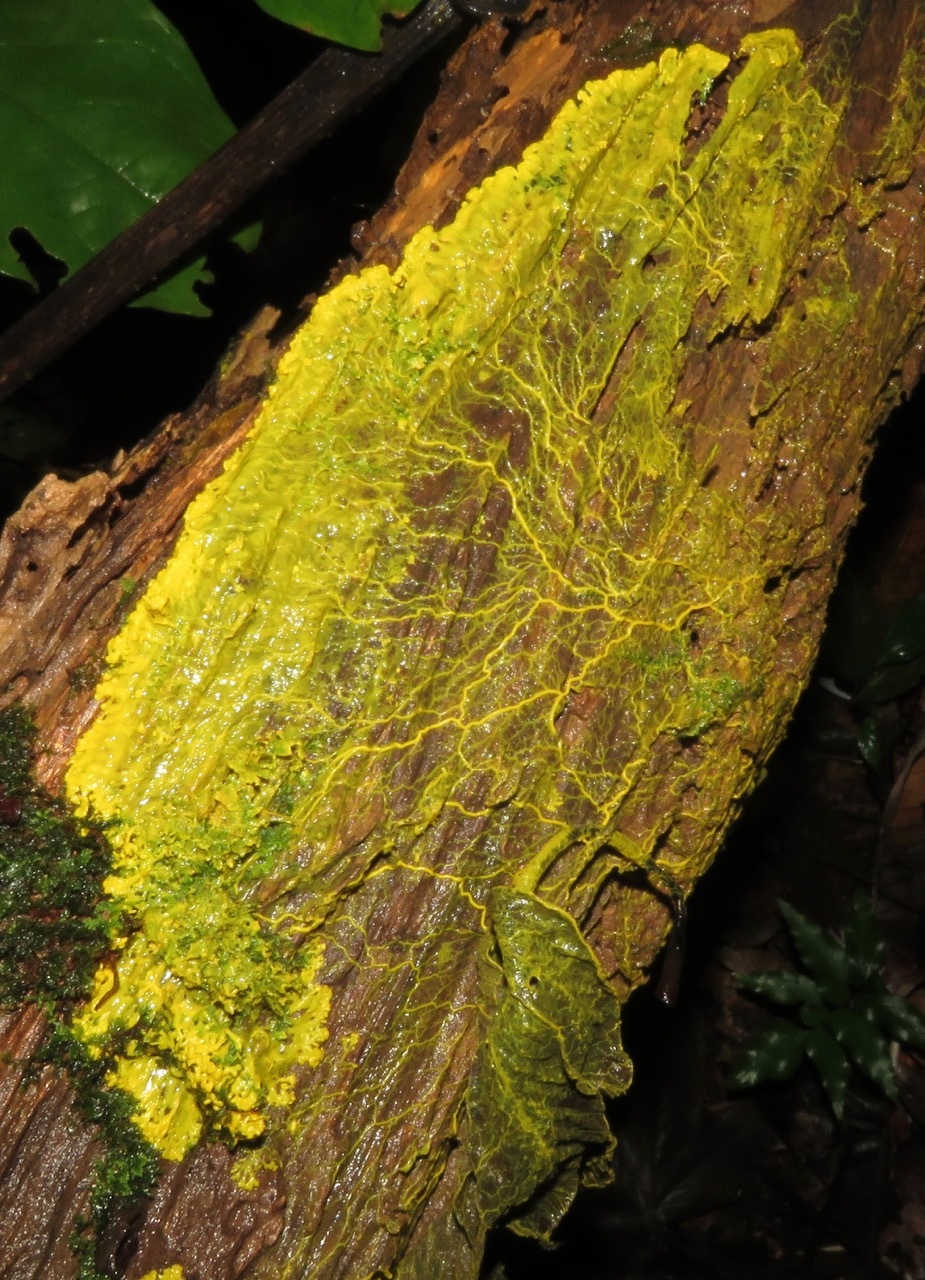
\includegraphics[scale=0.45]{images/Physarum_polycephalum_(3).jpg}
	\caption[Plasmodium of Physarum polycephalum]{Plasmodium of Physarum polycephalum (R. Hoyer/Wikipedia. Creative Commons)}
	\label{fig:plasmodianpp}
\end{figure}

\subsubsection{Characteristics}
Lorem ipsum dolor sit amet, consetetur sadipscing elitr, sed diam nonumy eirmod tempor invidunt ut labore et dolore magna aliquyam erat, sed diam voluptua. At vero eos et accusam et justo duo dolores et ea rebum. Stet clita kasd gubergren, no sea takimata sanctus est Lorem ipsum dolor sit amet. Lorem ipsum dolor sit amet, consetetur sadipscing elitr, sed diam nonumy eirmod tempor invidunt ut labore et dolore magna aliquyam erat, sed diam voluptua. At vero eos et accusam et justo duo dolores et ea rebum. Stet clita kasd gubergren, no sea takimata sanctus est Lorem ipsum dolor sit amet. Lorem ipsum dolor sit amet, consetetur sadipscing elitr, sed diam nonumy eirmod tempor invidunt ut labore et dolore magna aliquyam erat, sed diam voluptua. At vero eos et accusam et justo duo dolores et ea rebum. Stet clita kasd gubergren, no sea takimata sanctus est Lorem ipsum dolor sit amet.  \\\\Duis autem vel eum iriure dolor in hendrerit in vulputate velit esse molestie consequat, vel illum dolore eu feugiat nulla facilisis at vero eros et accumsan et iusto odio dignissim qui blandit praesent luptatum zzril delenit augue duis dolore te feugait nulla facilisi. Lorem ipsum dolor sit amet, consectetuer adipiscing elit, sed diam nonummy nibh euismod tincidunt ut laoreet dolore magna aliquam erat volutpat.\\\\Ut wisi enim ad minim veniam, quis nostrud exerci tation ullamcorper suscipit lobortis nisl ut aliquip ex ea commodo consequat. Duis autem vel eum iriure dolor in hendrerit in vulputate velit esse.

\subsubsection{Distribution}
Lorem ipsum dolor sit amet, consetetur sadipscing elitr, sed diam nonumy eirmod tempor invidunt ut labore et dolore magna aliquyam erat, sed diam voluptua. At vero eos et accusam et justo duo dolores et ea rebum. Stet clita kasd gubergren, no sea takimata sanctus est Lorem ipsum dolor sit amet. Lorem ipsum dolor sit amet, consetetur sadipscing elitr, sed diam nonumy eirmod tempor invidunt ut labore et dolore magna aliquyam erat, sed diam voluptua. At vero eos et accusam et justo duo dolores et ea rebum.
hia. 

\section{Life Cycle}
Lorem ipsum dolor sit amet, consetetur sadipscing elitr, sed diam nonumy eirmod tempor invidunt ut labore et dolore magna aliquyam erat, sed diam voluptua. At vero eos et accusam et justo duo dolores et ea rebum. Stet clita kasd gubergren, no sea takimata sanctus est Lorem ipsum dolor sit amet. Lorem ipsum dolor sit amet, consetetur sadipscing elitr, sed diam nonumy eirmod tempor invidunt ut labore et dolore magna aliquyam erat, sed diam voluptua. At vero eos et accusam et justo duo dolores et ea rebum. Stet clita kasd gubergren, no sea takimata sanctus est Lorem ipsum dolor sit amet. Lorem ipsum dolor sit amet, consetetur sadipscing elitr, sed diam nonumy eirmod tempor invidunt ut labore et dolore magna aliquyam erat, sed diam voluptua. At vero eos et accusam et justo duo dolores et ea rebum. Stet clita kasd gubergren, no sea takimata sanctus est Lorem ipsum dolor sit amet.  \\\\Duis autem vel eum iriure dolor in hendrerit in vulputate velit esse molestie consequat, vel illum dolore eu feugiat nulla facilisis at vero eros et accumsan et iusto odio dignissim qui blandit praesent luptatum zzril delenit augue duis dolore te feugait nulla facilisi. Lorem ipsum dolor sit amet, consectetuer adipiscing elit, sed diam nonummy nibh euismod tincidunt ut laoreet dolore magna aliquam erat volutpat.\\\\Ut wisi enim ad minim veniam, quis nostrud exerci tation ullamcorper suscipit lobortis nisl ut aliquip ex ea commodo consequat. Duis autem vel eum iriure dolor in hendrerit in vulputate velit esse.

\chapter{State of the Art}
\label{sec:relatedwork}
%This section talks about that which is retelling in video games
\section{Retelling games}

Game retelling is the act of reconstructing a past play experience into a new form whether through storytelling, video, illustration, or another medium. It is a way of making sense of what happened during play, translating fleeting moments into shareable narratives. In analog games like TTRPGs, where much of the story unfolds through improvisation and player interaction, retelling can serve many purposes. It preserves memories, communicates the experience to others, and allows for reflection on the themes, decisions, and dynamics that emerged. Whether casually recounted around a table, written into detailed session reports, or adapted into comics and podcasts, game retellings are always interpretive. They emphasize certain moments over others, shift the tone or point of view, and reshape nonlinear, messy play into something structured and communicable.

This process is not only about preserving content it is also an act of authorship. As soon as one begins to retell a game, choices are made about what matters, what is meaningful, and what should be retold. In doing so, the reteller inevitably reshapes the story, turning play into narrative. This transformation forms the foundation for deeper theoretical approaches to game retelling, including those that consider it a form of critique, reflection, or creative reinterpretation. This is double important when it comes to TTRPGs as these are games that are normally are not well recorded and live fully in the minds of the players with a couple spares notes on paper floating in the group.

Recapping is also a form of retelling. Many ongoing TV shows, series, anime, comic books, etc. tend to start each episode with a retelling of the previous episodes. Focusing only on the important aspects and leaving out a lot of the scenes. This is done in an attempt to reengage the watcher/reader and to remind them of the flow of the story so that they understand the story better. The same counts for TTRPG group who are part of a larger story that lasts numerous sessions separated by time. This is done in an attempt to restructure the story and make it clear to all the players to understand where they are in the story.

Retelling a game session, especially a TTRPG like Dungeons & Dragons, is not merely an act of documentation. It is a creative, interpretative, and often critical practice. In transforming a game  play experience into a new form, such as a comic book, the storyteller engages in a process of selection, transformation, and framing. This process raises questions not only about how stories are told, but also about what aspects of play are preserved, emphasized, or reimagined. After all a big part of the identity of a TTRPG is its rules and game play structures. Keeping play and the experience of playing in a retelling of a TTRPG is a key factor of conveying the story and the player experience.

Eladhari introduces the concept of game retelling as the fourth layer of narrative. According to Eladhari, this layer exists beyond the embedded, emergent, and interpreted narratives that typically characterize game storytelling. The fourth layer is concerned with post-play reflection and reinterpretation. It allows players, designers, or critics to re-engage with a game experience after the fact, often through a different medium (Eladhari 2018). In this view, retelling is not just about conveying what happened in the game, it is also about creating space for analysis, critique, or emotional processing.

Sych expands on this concept by arguing that critical game retellings can serve as a bridge between personal experience and broader thematic exploration. By combining Eladhari’s fourth layer with the idea of “breaking the fourth wall” Sych shows how retellings can expose the mechanics, social dynamics, and ethical tensions of gameplay itself (Sych 2022). This is particularly relevant in TTRPGs, where storytelling and rules are deeply intertwined, and where players often make decisions that reflect not just in-game motivations, but also real-world values and group norms.

Moreover, game retelling in this form invites consideration of what is lost and what is gained in translation. Elements like humor, tension, or spontaneity may be flattened or reshaped, while the visual format offers new tools, framing, symbolism, visual rhythm, to convey meaning. As Eladhari notes, retelling is not just representational it is generative. It produces new readings, new interpretations, and sometimes even new stories.

Finally, comic-based retelling also offers a lens into how different types of player interaction, such as roleplay, exposition, and rule engagement, manifest in a visual medium. The project thus becomes a way to explore not only how games are retold, but also how different aspects of a game are retold by artificial intelligence.


% Re-Tellings: The Fourth Layer of Narrative as an Instrument for Critique - Mirjam Palosaari Eladhari
% When the Fourth Layer Meets the Fourth Wall: The Case for Critical Game Retellings - Steven Sych

%This section showcases examples of retelling in video games
\subsection{Examples of TTRPG retellings}
%Adventure Zone (Comic) & Critical Role (Cartoon)

%This section showcases examples 1of AI based retelling/storytelling
\subsection{Artificial Intelligence as a Reteller/storyteller}
%AI Comic factory and The Finals commentator

%In this section we will look at comic studies and use that as a basis for the project
\section{Comic books}
%Understanding Comics (Scott McCloud) and Comics and Sequential Art (Will Eisner)	
Making Comic Books is an art form on its own and to understand how to generate a comic book with AI we need to understand how comic books function as an artefact: How they are made; How they are structured; How they are read; And what comic books are. This section will look at comic book studies to create a better understanding of comic book creation.

Comic books are a sequential art form\cite{eisner2008comics}. When you take a comic book panel and look at it outside of the context of other panels it is just an image. But when you place them side by side in a sequential order the pictures become a comic book \ref{fig:SequentialArt}. Looking at the image we can see that an image of a man holding its hat is just a man holding a hat. But when you place two images of a man holding his hat side by side we can see that it creates a motion of tipping his hat. The panels create an effect of change, an effect of time passing. The space between the panels of comic book panels creates a concept of time in stationary images. 

\begin{figure}[!htp]
	\centering
	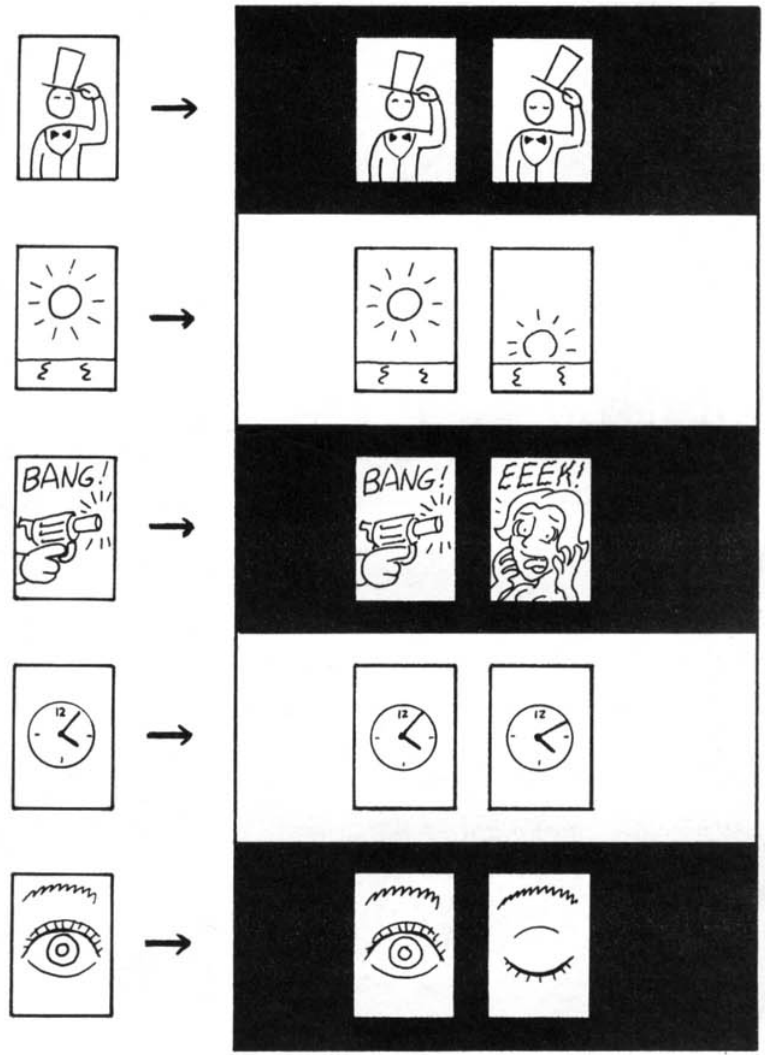
\includegraphics[scale=0.45]{images/SequentalArtUnderstandingComicPage5.png}
	\caption[Sequential Art]{Sequential Art page 5 \cite{mccloud1993understanding}}
	\label{fig:SequentialArt}
\end{figure}

In terms of art style there are many different flavours of comic books. Most people would think of a classic comic book they read as a child. But there are many more. Manga uses grey scale and generally follow a panel structure. American comics mostly are full colour and follow a panel structure. Manhwa/Webcomics are in mostly in full colour but are read from top to bottom by scrolling and are primarily read on the web. And these are just some generic descriptions of comic book art style, there are many unique styles out there like Sin City style (REF) and David Finch's art style (REF). Some comics even break the whole concept of panels and use whole pages as panels. Or place panels in panels. Or have panels that are not rectangular, but crooked, round, bend or anything else (Sandman). And some do not even use panels at all but make use of emptiness or use the same character on a long frame multiple time creating a concept of time as you read left to right. The important take away here is that comic books are not just one style, but many different styles.

Iconography is essential to many comic books to communicate those things that can not be easily spoken or written down. In the world of manga we call this unspoken communication \textit{Manpu} \ref{fig:Iconography}. To quote Matt Alt \textit{ Manpu "speak" what can't be easily spoken (or written) in words} \cite{GigaTown}. "ZZZ" to indicate someone is snoring or sleeping, a circle with starts and birds above a characters head indicate a state of unconsciousness by an impact of sorts, pages being torn of a calendar indicate time passing and one of my favourite making an L with your thumb and index finger and placing it under you chin to indicate deep thought (or the one I do not like where it represent people acting cool). 

\begin{figure}[!htp]
	\centering
	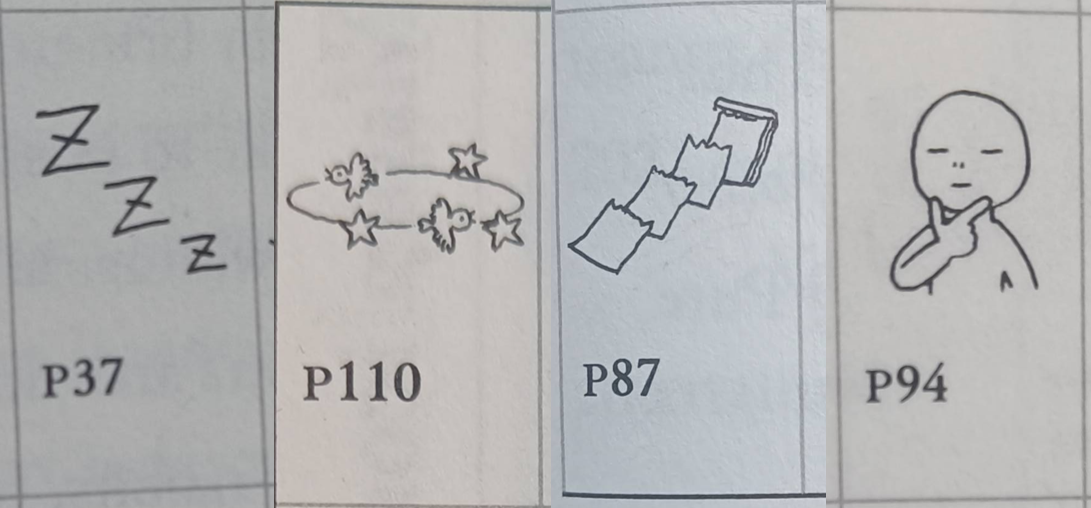
\includegraphics[scale=0.45]{images/IconographyGigaTown.png}
	\caption[Iconography]{Iconography \cite{GigaTown}}
	\label{fig:Iconography}
\end{figure}

Text in comic books are most 


So what did we learn from this? And what can we take with us for the artefact creation?
\begin{enumerate}
    \item Time in comic books. As time passes in between comic book panels we need to make sure that the AI generated comic book has a clear time line. The AI needs to be able to use the time line of the story and how it is told. Connecting panels to each other and create a feeling of time passing.
    \item Different panel styles. As we look at the different styles of panels that comic books use we need to ask ourselves to what extend the panel structure is important in an exploratory retelling artefact of games like the one made for this thesis. The panel structure is primarily an artistic expression of the greater whole of the comic book and the story it tells. The artefact is going to need a structured system to generate panels and it shouldn't have too much freedom to come up with panel structures as this will most likely take away from the retelling of the story of not done very well.
    \item Art start. As 
    \item Text in comic books
    \item Iconography
\end{enumerate}


\subsection{Comic Book take aways}

%In this section we will look at the different AI models and why I chose them
\section{AI models}
There are many different AI models floating around the internet that could be used as part of the artefact that was made for this thesis. To choice which model to use this chapter talks about different models and why they were chosen for this thesis. In the end Mistral has been chosen as the large language model, FLUX.1 has been chosen for the image generation and Whisper has been chosen for the audio transcription model.

The requirements where these models where chosen on were:
\begin{itemize}
	\item Open source
	\item Locally runnable
	\item Good enough performance
	\item Ethical considerations as disclosed in section \ref{AIethics}
\end{itemize}
\subsection{Large Language Models}

Picking a suitable Large Language Model for the project is a quite the impossible task as models keep changing rapidly and new models are released every day. There are many academic papers out there discussing models and their performance, usage and more \cite{2024arXiv240201687A,chang2024survey,hadi2023survey,zhao2023survey}. However all of these are already more than a year old and as models are changing so fast most of those papers are already outdated, however still very useful. As this paper is not an analysis of AI models but a practical thesis I have asked ChatGPT-4-turbo to give me a list of models with their pros and cons and asked it to make me a table for Latex with the information. The prompts that I used: \textit{I would like to have a table with a comparison of the top 10 large language models. Show the pro's and cons of the models. Add if they are open source and locally runnable.} Followed by: \textit{Can you convert that table to Latex code?}. The results can be seen in table \ref{tbl:ModelComparison}, the latex code had to be modified to fit the page.

Even here we can see that the models are out of date. Gemini 1.5 Pro is not the latest model as Gemini 2.5 is already released, and LLaMA 3.1 is not the latest model as LLaMA 4 is already released. However, the table does give a good overview of the models that are available and their pros and cons. Primarily the question if they are open source and can be run locally. I used this method not because I see it as a academic valuable method but because I want to use technology and see how useful it could be for academia. Looking at this small experiment we can see that it could be useful, however the data is very outdated and not very useful. It does point us in the correct direction and gives us a good overview of the models that are available.

\begin{table}[ht!]
\centering
\resizebox{\textwidth}{!}{%
\begin{tabular}{|l|l|p{5cm}|p{5cm}|c|c|}
\hline
\textbf{Model Name} & \textbf{Developer} & \textbf{Pros} & \textbf{Cons} & \textbf{Open Source} & \textbf{Locally Runnable} \\
\hline
GPT-4o & OpenAI & 
Multimodal (text, image, audio); fast and versatile & 
Occasional hallucinations; high compute needed & 
No & No \\
\hline
Claude 3.5 Sonnet & Anthropic & 
Safety-focused; handles long contexts; natural responses & 
Slower; closed API only & 
No & No \\
\hline
Gemini 1.5 Pro & Google DeepMind & 
Strong multimodal support; integrates Google ecosystem & 
Resource-heavy; limited open variants & 
No & No \\
\hline
LLaMA 3.1 & Meta AI & 
Open-source; good at translation and code & 
Requires technical expertise; energy-intensive & 
Yes & Yes \\
\hline
Mistral Large 2 & Mistral AI & 
Strong reasoning and code generation; long contexts & 
Commercial license; proprietary & 
No & Limited (license) \\
\hline
DeepSeek-R1 & DeepSeek & 
Multilingual support; efficient & 
Limited adoption; less documented & 
No & No \\
\hline
Mixtral & Mistral AI & 
Efficient Mixture of Experts; open-source & 
Shorter context; niche usage & 
Yes & Yes \\
\hline
Grok 3 & xAI & 
Good social media integration; open-source focus & 
Requires subscription; limited distribution & 
Yes & Possibly (limited) \\
\hline
Command R+ & Cohere & 
Up-to-date info retrieval; good conversational skills & 
Limited multimodal support & 
No & No \\
\hline
Phi-2 & Microsoft & 
Open-source; efficient size/performance & 
Limited multimodal support; some bias concerns & 
Yes & Yes \\
\hline
\end{tabular}
}
\captionof{table}{Comparison table of 10 LLM's by ChatGPT-4-turbo}\label{tbl:ModelComparison}
\end{table}\noindent

Looking at the options provided we can quickly cut out most of the models as they are not open source and there is no possibility of running them locally. The models that are left are LLaMA, Mixtral and Phi. Out of these 3 models the choice is easy as Mixtral is the only options. Even do the other two models are open source, they are still owned by large American corporations (Microsoft and Meta) which are from personal point of view out of the question to use (More on this in \ref{AIethics}). Mistral is an privately owned and French company.

\subsection{Image generation models} 

\cite{bie2024renaissance}

%Talk about Stable Diffusion, Llama 3.1-8B and Whisper and why I chose them. Also talk about other models and why I did not choose them.

%In this section I will talk about the ethical consideration around AI usage.
\section{AI ethics} \label{AIethics}
Hello
%The Ethics of AI in games. – Melhart et al.
% Building ethics into artificial intelligence. – Yu et al.
% Deep Learning for Coders with Fastai and Pytorch: AI Applications Without a PhD – Jeremy Howard & Sylvain Gugger
% The ethics of Artificial Intelligence – Nick Bostrom & Eliezer Yudkowsky
% Think about stepping on the toes of artists and writers.

\section{The art of AI prompting}
Writing AI prompts is not something you can properly do without thinking about it. Writing proper prompts is a lot like writing code where you need to iterate over the instructions you give the computer to do what you want it to do. It is also know as prompt engineering. There are a lot of nuances to writing prompts and hidden tricks and commands to instruct an AI to get an AI to do exactly what you want it to do. This section discusses the basics of AI prompting and how they have been used in the artefact.

\cite{dang2022prompt}
%https://scholar.google.com/scholar?hl=nl&as_sdt=0%2C5&q=How+to+prompt+ai&btnG=

\section{Three primary forms of player interaction}
GPT:

Dungeons and Dragons sessions have three primary forms of player interaction: roleplay, exposition, and rule interaction. These three forms are distinctly different, and in this project they will be used to analyze different parts of the generated comic book to see if the system is better at certain parts.

Roleplay is when players and the dungeon master talk to each other while taking on the role of their characters. The dungeon master often juggles multiple roles, shifting between NPCs as needed. This kind of interaction mostly happens in-character and aligns with what game researchers call the narrativist mode from GNS theory, where the focus is on creating a story together (Edwards 2001). It also maps onto what is known in RPG studies as in-character talk, one of the core communication styles during play (Bowman 2010).

Exposition is when the dungeon master describes a situation, a location, or the mood of a scene. It is about creating a vivid image of what is happening in the game. This is not necessarily roleplaying, but it is key to setting the stage. It sits somewhere between narrativist and simulationist modes in GNS theory, and would be considered out-of-character talk, since it is often descriptive rather than spoken as a character (Bowman 2010).

Rule interaction is where the game mechanics kick in. This is when players roll dice and use other rules of the system to resolve conflicts, check if they hit an enemy, try to jump through a window, activate an ability, or make a persuasion check to convince someone that they are innocent. These moments are very gamist in nature. They are about winning challenges through the rules of the system. In terms of communication, this fits under meta talk, which includes discussing rules, tactics, or numbers, often from outside the fiction (Bowman 2010).

These three types of interaction not only shape how players experience the game, but also how that session is interpreted when turning it into a comic. Based on these three categories the final comic book result will be analyzed to see what is the difference to retelling these parts and to see what the differce is inbetween generation.

\chapter{Background and Methods}
\label{sec:methods}
\label{sec:Implementation}
This chapter iterative design process of the artefact.
\section{My Topic}


\section{Coding with Python}
Python was the only language used in this project. This was chosen as Python is the go to language for programming with AI models (REF) and all major(if not all) models have python support.

Specifically python version 3.12.3 running on a the Windows Subsystem for Linux version 2 (WSL) running Ubuntu 24.04.2 LTS. WSL is a windows feature that allows you to run a Linux environment directly on Windows while in windows without having to run a virtual machine. You control the Linux distribution fully through the terminal.

\section{AI models}

\subsection{Whisper}

\subsection{Llama}

\subsection{Image generating models: Stable Diffusion}
The chosen image generation model is Stable Diffusion version stabilityai/stable-diffusion-xl-base-1.0 \cite{StableDiffusionGit}




\chapter{Artefact Development}
\label{sec:implementation}
\label{sec:Implementation}

\section{My Topic}
Lorem ipsum dolor sit amet, consetetur sadipscing elitr, sed diam nonumy eirmod tempor invidunt ut labore et dolore magna aliquyam erat, sed diam voluptua. At vero eos et accusam et justo duo dolores et ea rebum. Stet clita kasd gubergren, no sea takimata sanctus est Lorem ipsum dolor sit amet. Lorem ipsum dolor sit amet, consetetur sadipscing elitr, sed diam nonumy eirmod tempor invidunt ut labore et dolore magna aliquyam erat, sed diam voluptua. At vero eos et accusam et justo duo dolores et ea rebum. Stet clita kasd gubergren, no sea takimata sanctus est Lorem ipsum dolor sit amet. Lorem ipsum dolor sit amet, consetetur sadipscing elitr, sed diam nonumy eirmod tempor invidunt ut labore et dolore magna aliquyam erat, sed diam voluptua. At vero eos et accusam et.

\section{My Work}
Stet clita kasd gubergren, no sea takimata sanctus est Lorem ipsum dolor sit amet. Lorem ipsum dolor sit amet, consetetur sadipscing elitr, sed diam nonumy eirmod tempor invidunt ut labore et dolore magna aliquyam erat, sed diam voluptua. At vero eos et accusam et.

\section{My Implementation}
Stet clita kasd gubergren, no sea takimata sanctus est Lorem ipsum dolor sit amet. Lorem ipsum dolor sit amet, consetetur sadipscing elitr, sed diam nonumy eirmod tempor invidunt ut labore et dolore magna aliquyam erat, sed diam voluptua. At vero eos et accusam et.

\subsection{Initialization}
Stet clita kasd gubergren, no sea takimata sanctus est Lorem ipsum dolor sit amet. Lorem ipsum dolor sit amet, consetetur sadipscing elitr, sed diam nonumy eirmod tempor invidunt ut labore et dolore magna aliquyam erat, sed diam voluptua. At vero eos et accusam et.

\subsection{Setup}
HStet clita kasd gubergren, no sea takimata sanctus est Lorem ipsum dolor sit amet. Lorem ipsum dolor sit amet, consetetur sadipscing elitr, sed diam nonumy eirmod tempor invidunt ut labore et dolore magna aliquyam erat, sed diam voluptua. At vero eos et accusam et.

\subsection{Simulation Process}
Stet clita kasd gubergren, no sea takimata sanctus est Lorem ipsum dolor sit amet. Lorem ipsum dolor sit amet, consetetur sadipscing elitr, sed diam nonumy eirmod tempor invidunt ut labore et dolore magna aliquyam erat, sed diam voluptua. At vero eos et accusam et. Stet clita kasd gubergren, no sea takimata sanctus est Lorem ipsum dolor sit amet. Lorem ipsum dolor sit amet, consetetur sadipscing elitr, sed diam nonumy eirmod tempor invidunt ut labore et dolore magna aliquyam erat, sed diam voluptua. At vero eos et accusam et.




\chapter{Experiments}
\label{sec:experiments}

\section{Experiments and Simulations}

\section{The minimal viable product}
The minimal viable product (MVP) is a version of a new product that includes only the essential features necessary to meet the needs for initial testing. The goal of an MVP is to validate the product idea with minimal resources and gather feedback for future development. In figure \ref{fig:MVP} you can see the result of the MVP and in figure \ref{fig:MVPpipeline} you can see the pipeline that is used for the MVP.

\begin{figure}[!htp]
    \centering
    \includegraphics[scale=0.2]{images/mvpTTRPGtoComic.png}
    \caption[The minimal viable product]{The minimal viable product}
    \label{fig:MVP}
\end{figure}

\subsubsection{MVP pipeline}
The MVP pipeline has 4 steps of processing to go from audio recording to comic book. First Whisper Turbo transcribes the audio recording to raw text. Then Llama 3.1 converts the text to a comic book script. The script is then processed by Stable Diffusion XL to generate the comic book panels. Finally, the panels are assembled into a comic book format using a custom python script. The pipeline is shown in figure \ref{fig:MVPpipeline}. The audio recording is a single track recording of a tabletop role-playing game session. The prompt used for Llama can be seen in listing \ref{lst:MPVLlamaprompt}. This prompt generates a description of the panel art and a line of dialogue or narration for each panel. The output is a JSON array of objects, where each object contains the panel art description and the text. The panel art description is then given to Stable Diffusion XL to generate the image with no other instructions. The text is used as a caption for the image. The images are then assembled into a comic book format using a custom python script which generates a PDF file with the images and captions.

\begin{lstlisting}[style=jsonstyle, caption={Prompt for Comic Book Script Generation}, label={lst:MPVLlamaprompt}]
You are given a segment of a Dungeons & Dragons session transcript:

Session Content:
{content}

Your task is to transform this into a comic book script, broken down into individual panels.

Each panel must include:
- A detailed visual description suitable for image generation (key: "panel art")
- A line of dialogue or narration (key: "text")

Instructions:
- Structure the output as a JSON array of objects.
- Each object must contain exactly two keys:
- "panel art": A vivid, standalone description of the panel art. Include setting, characters, action, and mood.
- "text": A single line of spoken dialogue or narration. Rephrase as a proper sentence if needed, but keep the meaning true to the original session.
- Process the entire input and split it into as many panels as necessary.
- Do **not** include any additional explanation, commentary, or text outside of the JSON array.

Output only a valid JSON array. Example format:

[
{
    "panel art": "A dimly lit tavern filled with laughing patrons. Magnus, a red-bearded human, clinks mugs with Taco and Merle at a wooden table.",
    "text": "So our story begins with the three of you sitting at this tavern."
},
{
    "panel art": "Close-up of Magnus, his face lit by candlelight, a sheepish grin on his face.",
    "text": "Nobody wants chairs anymore. Everyones into wrought iron now."
}
]
\end{lstlisting}

\subsection{Lessons learned}
The MVP was a success in terms of validating the product idea and gathering valuable knowledge about the product requirements and limitations. In this section lessons learned are described in detail and it is discussed how these lesson will be implemented in the next iteration of the product.

\subsubsection{Art}
The first thing one might see when looking at the MVP output is the art. The art quality is low, it is not very detailed, the characters are not very expressive and the art style is very inconsistent. There are also a lot of generative AI artifacts, like weird faces and inconsistent human anatomy. Furthermore all these panels are situated in the same tavern, but the there is no consistent setting. All these panels also describe 4 different characters and but there is no consistent character design between panels.

\subsubsection{Text}
The text has one obvious flaw of clipping outside of the image which is something that needs to be fixed. Other then that when reading the text it is noticeable that it is not really character dialogue, but things the players are saying. Some of the text is player to player dialogue and not in character dialogue which is something that needs to be filtered out. The text also does not make any since in term of story structure. These are just lines of text.

Looking the entire transcription of the tabletop role-playing game session it can quickly be seen that there is no structure to the text, making it extremely difficult for an LLM to make anything meaningful out of it. Figure X is a expert of the transcript where you can see that it is just a consistent stream of text without any structure.

\subsubsection{Composition}
All the panels have a similar camera angle and composition.

\subsection{Solutions}
In this section possible solutions are discussed which will be implemented for the next iteration of the product. The goal is to improve the quality of the art, text and composition of the comic book panels.

\subsubsection{Art}
Stable Diffusion is a pre-trained model that is made to work for any art style, to create a consistent art style you could write a art style prompt, however this creates issues with the token limit that stable diffusion has. The proper way to do this is by using a loRA (Low-Rank Adaptation). LoRAs are a way to fine-tune a pre-trained model on a specific task or domain. In this case, a LoRA can be trained on a specific art style to create a consistent art style for the comic book panels. This will also allow for more detailed and expressive characters. The LoRA can be trained on a dataset of comic book panels in the desired art style. The LoRA can then be used in Stable Diffusion to generate the comic book panels with the desired art style. However since training a LoRA is outside of the scope of this project a pre-trained LoRA from civitai.com will be used. This also comes with the benefit that any LoRA can be used to generate any art style wanted by the user.

\subsubsection{Character consistency}
To create consistent characters between panels there are 5 different approaches that can be taken. LoRA's can be used for each character creating a very consistent character design. This does require each character to have a LoRA trained on it meaning that you need to have art of the character to start with. This would also mean that the images would be generated with multiple AI's generating images and then having to combine them. 
The second option would be image-to-image reference chaining. With this method you give SDXL a reference image of the character and then generate the panel with the character art as a reference. 

The easiest and least consistent manner would be to use consistent prompting. This means that you give the same prompt for each panel with the character description in it. This will however not create a very consistent character as each iteration of the prompt will interpret the prompt differently. Resulting in many different smaller inconsistencies. This however would be a good step if the other methods would be too time consuming to implement. It would most likely require two iterations of generating the image, one for the character and one for the panel art. As the number of tokens in the prompt would be too high to generate the panel art and character art in one go.

Inpainting is a technique where you alter part of an image so that it fits your desired effect. You select an area of the image and then fill it in with a new image, generated by AI. This gives you a way to control very specific parts of an image and finetune an image. Normally this requires a lot of manual work where you have to cut out the area which has to be painted in. It would however be possible to use computer vision to detect the character in the image and then use that as a mask for the inpainting. This might result in a very good solution, but there are potential issues with multiple characters in the same panel.

Lastly an option could be using ControlNet. This is a technique where you use a pose reference images to control the pose of the character in the image.

In the end it would most likely be best to use most of the above techniques in combination to create the best possible result. Create a LoRA to have consistent character art, use inpainting to place the art on top of the panel art and use ControlNet to control the pose of the character. 
\subsubsection{Scene consistency}
In the current comic page of the MVP each scene is taking place in the same tavern, but the tavern is not consistent between panels. Most solutions given in the previous section on character consistency could be used here as well, however as there are way more variables possible for locations creating a LoRA is impossible and would defeat the purpose of using AI. You could however let AI create images of a tavern and the use those images as reference materials for future uses of that tavern. Meaning you need to keep track of scenes and locations so that you can bring back the same panels in later parts of the comic book. 

\subsubsection{Text}
To fix the text that is in the panels of the comic books the first step would be to fix the transcript of the game session. As is always the case with AI: Garbage in is garbage out. Fixing the transcript will also have effect on the other parts of the comic book, as there will be a clearer structure to the text which can be used in a better way to generate images and create structure between panels. To fix the transcription there are a few that need to be taken.

After transcribing the audio recording with whisper there are 3 steps we can take to increase the usability of the text. First we need to use a Punctuation and Capitalization Restoration model to fix the text by adding punctuation and capitalization to the text. This will make the text more readable and easier to understand. The second step would be to use Speaker Diarization to identify the different speakers in the text. This will benefit with knowing who said what at which time and allows to have accurate charact dialogue. Furthermore this makes it so that the Game Master can be identified as someone who plays multiple characters. A tool to do this is Pyannote Audio, an open-source toolkit written in Python for speaker diarization. Lastly combine the cleaned up whisper transcription with the speaker diarization to create a structured text file.

The next step is to then use an LLM to check all the text and identify what is character to character and what is player to player speech. Creating a clear divide between what does and what does not belong in the comic book. For the game master the same thing needs to happen, but then it is required to identify which character they are playing at that moment. Then an LLM would need to convert the text into real sentences which make sense in the context of the scene as something a someone in the English language would say.

\begin{figure}[!htp]
	\centering
	\includegraphics[scale=0.1]{images/mvpTTRPGtoComic.png}
	\caption[pipeline for the minimal viable product] {The minimal viable product pipeline}
	\label{fig:MVPpipeline}
\end{figure}

\subsection{The minimal viable product}

\section{Small experiments}

\subsection{The language of TTRPGs}
Models like Whisper are trained on a wide variety of audio data, however this is primarily normal language usage. Because of this I anticipate that there will be a large issue with transcribing many fantasy words and terms, thus a small experiment has been done to identify if this is truly a problem. For this experiment 10 fantasy creature names have been recorded and whisper transcribed these 10 names. Only 1 out of the 10 names were transcribed correctly and 2 out of 10 where almost correct \ref{tab:monster_names}. This is inaccuracy is a big issue when transcribing any fantasy game session as it will interfere with many important key moments and key names during a session/campaign. When the group meets a monster called a "Slaad" and Whisper transcribes this as "Nod" it will quite confusing to understand what is going on in the story.

To generate a accurate transcription of the names a custom model needs to be trained on specific fantasy words and terms, however this is way outside of the scope of this thesis. In addition it is also very difficult as Fantasy names are fantasy names for a reason and people can just come up with new names all the time. Integrating thousands of names however could still be valuable as it will most likely catch most cases.
\begin{table}[h!]
\centering
\begin{tabular}{|l|l|}
\hline
\textbf{Correct Name} & \textbf{Transcribed name} \\
\hline
Owlbear    & Halber     \\
Goblin     & Goblin     \\
Rakshasa   & Raksasa    \\
Dracolich  & Draco Lich \\
Quasit     & Kwasi      \\
Slaad      & Nod        \\
Drow       & Drought    \\
Illithid   & Illidan    \\
Cambion    & Kempion    \\
Ankheg     & Hank Man   \\
\hline
\end{tabular}
\caption{Comparison of monster names and whisper transcribed versions}
\label{tab:monster_names}
\end{table}

\section{Generating the comic book script}
The iterative design process of generating the comic book script after the MVP version was a crucial step to improve the quality of the comic book panels. From having a one-shot approach where we gave the entire transcript to the LLama 3.1 model, we moved to an adaptive panel generator which has a structured approach to data and keeps track of the context. In this section all the iterative steps are described and what did and did not work in chronological order.

\subsubsection{MVP}
For the MVP of the artefact the entire transcript of the tabletop role-playing game session was given to Llama 3.1 and see what it would generate. The LLM was asked: "You are given a Dungeons and Dragons session transcript. Convert it into a comic book script." This resulted in two results: The LLM crashed as the token limit was exceeded or it gave things that had nothing to do to with the input and hallucinated everything. A quick fix to this was to cut the transcript into smaller chunks of text which resulted in an interesting result as it actually gave a comic book script. It was given 2 scenes of text which where hand cut out of the transcript. However as the LLM was not instructed to give a structured output it was useless as every time the program was run it would give a different output. The last step was to create a structured prompt for the LLM which is the prompt in \ref{lst:MPVLlamaprompt}. This resulted in a consistent JSON format output which could then be used to generate images.

\subsubsection{Cleaning up the transcript}
When you feed an audio recording to Whisper it transcribes the audio as one long sentence. There is no punctation or any idea of sentences structure. This way it is impossible to keep track of who said what and when. To fix this the transcript needs to be cleaned up. The first step is to use a Punctuation and Capitalization Restoration model \cite{guhr-EtAl:2021:fullstop} to add punctuation and capitalization to the text. This will make the text more readable and easier to understand for an LLM. The second step is to use Speaker Diarization to identify the different speakers in the text. The tool used to do this was pyannote 3.1 \cite{Bredin23,Plaquet23}, an open source python library which is super easy to use and broadly used by people (15 million download per month). Lastly combine the cleaned up whisper transcription with the speaker diarization to create a structured JSON file. This new transcript file \ref{lst:sessionTrarnscriptJSON} is what created the foundation for the entire comic book generator.

\begin{lstlisting}[style=jsonstyle, caption={Session transcript JSON}, label={lst:sessionTrarnscriptJSON}]
{
    "panel_index": 0,
    "speaker": "SPEAKER_02",
    "text": "Our story actually starts with the three of you...",
    "start": 0.0,
    "end": 2.96
},
...
\end{lstlisting}

\subsubsection{Scene detection}

\subsubsection{Line based chunking}
Every line or every X lines

\subsubsection{LLM based chunking}
Scene cutting

\subsubsection{LLM based filtering}
Ask the LLM to decide if a line of text is player or character speech. Into giving it a chunk instead.

\subsubsection{Context aware LLM based chunking}

\subsubsection{Adaptive panel generating}

\chapter{Conclusion}
\label{sec:conclusion}
\section{Summary}
Lorem ipsum dolor sit amet, consetetur sadipscing elitr, sed diam nonumy eirmod tempor invidunt ut labore et dolore magna aliquyam erat, sed diam voluptua. At vero eos et accusam et justo duo dolores et ea rebum. Stet clita kasd gubergren, no sea takimata sanctus est Lorem ipsum dolor sit amet. Lorem ipsum dolor sit amet, consetetur sadipscing elitr, sed diam nonumy eirmod tempor invidunt ut labore et dolore magna aliquyam erat, sed diam voluptua. At vero eos et accusam et justo duo dolores et ea rebum. Stet clita kasd gubergren, no sea takimata sanctus est Lorem ipsum dolor sit amet.Lorem ipsum dolor sit amet, consetetur sadipscing elitr, sed diam nonumy eirmod tempor invidunt ut labore et dolore magna aliquyam erat, sed diam voluptua. At vero eos et accusam et justo duo dolores et ea rebum. Stet clita kasd gubergren, no sea takimata sanctus est Lorem ipsum dolor sit amet. Lorem ipsum dolor sit amet, consetetur sadipscing elitr, sed diam nonumy eirmod tempor invidunt ut labore et dolore magna aliquyam erat, sed diam voluptua. At vero eos et accusam et justo duo dolores et ea rebum. Stet clita kasd gubergren, no sea takimata sanctus est Lorem ipsum dolor sit amet.

\section{Further Work}
Lorem ipsum dolor sit amet, consetetur sadipscing elitr, sed diam nonumy eirmod tempor invidunt ut labore et dolore magna aliquyam erat, sed diam voluptua. At vero eos et accusam et justo duo dolores et ea rebum. Stet clita kasd gubergren, no sea takimata sanctus est Lorem ipsum dolor sit amet.

\subsection{Idea 1}
Lorem ipsum dolor sit amet, consetetur sadipscing elitr, sed diam nonumy eirmod tempor invidunt ut labore et dolore magna aliquyam erat, sed diam voluptua. At vero eos et accusam et justo duo dolores et ea rebum. Stet clita kasd gubergren, no sea takimata sanctus est Lorem ipsum dolor sit amet. Lorem ipsum dolor sit amet, consetetur sadipscing elitr, sed diam nonumy eirmod tempor invidunt ut labore et dolore magna aliquyam erat, sed diam voluptua. At vero eos et accusam et justo duo dolores et ea rebum. Stet clita kasd gubergren, no sea takimata sanctus est Lorem ipsum dolor sit amet.

\subsection{Idea 2}
Lorem ipsum dolor sit amet, consetetur sadipscing elitr, sed diam nonumy eirmod tempor invidunt ut labore et dolore magna aliquyam erat, sed diam voluptua. At vero eos et accusam et justo duo dolores et ea rebum. Stet clita kasd gubergren, no sea takimata sanctus est Lorem ipsum dolor sit amet. Lorem ipsum dolor sit amet, consetetur sadipscing elitr, sed diam nonumy eirmod tempor invidunt ut labore et dolore magna aliquyam erat, sed diam voluptua. At vero eos et accusam et justo duo dolores et ea rebum. Stet clita kasd gubergren, no sea takimata sanctus est Lorem ipsum dolor sit amet.


\newpage

\bibliographystyle{abbrv}
\addcontentsline{toc}{chapter}{Bibliography}
\bibliography{bibfile}

\newpage

\appendix
\addcontentsline{toc}{chapter}{APPENDICES}
\chapter{NetLogo Code}
\label{sec:appendix-netlogo}

\section{NetLogo Main}
\section{SISMO NetLogo Main Function}
\lstset{language=NetLogo}
\begin{lstlisting}
__includes["math_functions.nls" "setup.nls" "network-creation.nls" "a-star.nls"]
;; 6 breeds needed in total, 3 for slime mold (plasmodia, pseudopodia, tubes), 1 for food source and 2 for A* algorithm ( networkpoints, searchers)
breed [ plasmodia plasmodium ]
breed [ pseudopodia pseudopodium ]
;; The tubes are used to indicate the shortest path between the center and the feed source
breed [ tubes tube ]
;; foods represent the foodsources
breed [ foods food ]
;; the networkpoints and searchers are used for the a*algorithm
breed [ networkpoints networkpoint ]
breed [ searchers searcher ]

globals [
  ;; to control the form of the visible chemical field
  scale-factor
  ;; sets the probability for pseudopodia to hatch a new pseudopodium
  hatch-probability
]

pseudopodia-own[
  ;; stores the path in a list of lists with x y coordinates
  path-list
]

foods-own [
  ;; each food source should have an amount of nutrients
  nutrient-value
  ;; the chemical level describes the radius of the food source in which the pseudopodia can perceive the food
  chemical-level
  ;; for the visibility of the chemical field
  intensity
]

tubes-own [
  ;; stores the path in a list of lists with x y coordinates
  path-list
]

searchers-own [
  memory               ; Stores the path from the start node to here
  cost                 ; Stores the real cost from the start
  total-expected-cost  ; Stores the total exepcted cost from Start to the Goal that is being computed
  localization         ; The searchers position
  active?              ; is the searcher active? That is, we have reached the node, but we must consider it because its neighbors have not been explored
]

patches-own
[
  light-level ;; represents the light energy from all light sources
]

;; setup, defines where to place which component of the simulation at the beginning and initialize the global variables
to setup
  ;; clear-all calls the clearing functions like clear-globals etc.
  clear-all
  ;; set global variables
  set hatch-probability 0.15
  set scale-factor 10
  ;; call make functions to create breeds
  make-plasmodia
  make-foods amount-foodsources
  make-pseudopodia amount-pseudopodia
  ;; next line is responsible for the visibility of the chemical concentration in the air
  ask patches [ generate-field ]
  ;; Resets the tick counter to zero, sets up all plots, then updates all plots
  reset-ticks
end

to go
  ifelse any? foods with [ nutrient-value > 0 ]
  [
    ask foods[
      ;; There is a bug where food sources are created randomly and untraceable. This causes the pseudopodia to hang on this food source. Because it takes negative values and iterates forever. With this code this bug is fixed.
      if nutrient-value < 0 [ die ]
    ]
    ask pseudopodia
    [
      let foodsource one-of foods-here
      ifelse foodsource != nobody
      [
        let path-list-to-provide-to-tube path-list
        ask foodsource
        [
          if show-nutrient-value [set label nutrient-value]
          set nutrient-value nutrient-value - 1
          if nutrient-value = 0 [
            ;; create the network for the a star algorithm
            create-pseudopodia-network turtle-set turtles-on patch-ahead 0
            ;; get one pseudopodia on the foodsource to set the destination x,y coordinate for the a* algorithm
            let one-pseudopodia-here one-of pseudopodia-here
            run-a-star 0 0 ([xcor] of one-pseudopodia-here) ([ycor] of one-pseudopodia-here)
            die
          ]
        ]
        ;; calculates a random float number between 0 an 1
        if random-float 1 <= hatch-probability
        [
          ;; create new child from pseudopodia, replace the zeros in the path-list to indicate, that it is a copy
          hatch-pseudopodia 1
          [
            let new-path-list replace-zeros path-list
            set path-list new-path-list
          ]
        ]
      ]
      [
        ;; movment of the pseudopodia -> bounce of the wall, movement and sense chemotaxis from food
        bounce
        wiggle
        look-for-food
      ]
    ]
    ;; if the a * buildet a tube display it
    ask tubes[
      let i 0
      while [i < length path-list - 1]
      [
        let x-1 [xcor] of item i path-list
        let y-1 [ycor] of item i path-list
        setxy x-1 y-1
        let col [pcolor] of one-of neighbors
        set i i + 1
      ]
      die
    ]
    tick
  ]
  [
    stop
  ]
end

to look-for-food
  ;; find chemotaxis in the area of a food source
  let foodsource one-of foods in-radius 5
  if (foodsource != nobody)
  [
    ;; if there is chemotaxis ahead move towards the center
    face foodsource
  ]
end

to wiggle
  rt random 40
  lt random 40
  if not can-move? 1 [ rt 180 ]
  fd 1
  ;; create a new entry for the path list (with x and y coordinates and 0 because the step from this pseudopodia is new)
  let xycoordinate (list xcor ycor 0)
  set path-list insert-item (length path-list) path-list xycoordinate
end

to bounce
  ;; bounce off left and right walls
  if abs pxcor >= max-pxcor - 1
  [
    ;; if "at the end of the world" face towards center and move one forward
    face patch 0 0
    ;; move one forward otherwise it will get stuck at the edge of the world
    fd 1
  ]
  ;; bounce off top and bottom walls
  if abs pycor >= max-pycor - 1
  [
    ;; if "at the end of the world" face towards center and move one forward
    face patch 0 0
    ;; move one forward otherwise it will get stuck at the edge of the world
    fd 1
  ]
end
\end{lstlisting}

\section{SISMO NetLogo Setup}
\begin{lstlisting}
;;;;;;;;;;;;;;;;;;;;;;
;; Setup Procedures ;;
;;;;;;;;;;;;;;;;;;;;;;

;; create slime population
to make-plasmodia
  create-plasmodia 1
  [
    set size 5
    set shape "cloud"
    set color yellow
  ]
end

;; create pseudopodia
to make-pseudopodia [number]
  create-pseudopodia number
  [
    ;; for the pseudopias we need the same starting position as for the plasmodium. Because it spreads from the center
    set color yellow
    set shape "dot"
    set path-list []
    set path-list insert-item 0 path-list (list xcor ycor 0)
    pen-down
  ]
end

;; create food sources
to make-foods [ number ]
  create-foods number [
    set shape "circle 2"
    set color orange
    set size 2
    ;; create random coordinate https://ccl.northwestern.edu/netlogo/bind/primitive/random-float.html#:~:text=If%20you%20want%20to%20generate,4%20%2B%20random%2Dfloat%203%20.
    ;; If you want to generate a random number between a custom range, you can use the following format: minnumber + (random-float (maxnumber - minnumber))
    let randomxcoord (min-pxcor + 3) + (random-float ((max-pxcor - 3) - (min-pxcor + 3)))
    let randomycoord (min-pycor + 3) + (random-float ((max-pycor - 3) - (min-pycor + 3)))
    setxy randomxcoord randomycoord
    set nutrient-value 50 + (random (150 - 50))
    set chemical-level 23
    set intensity 50
    set label-color red
  ]
end

;; patch procedure
to generate-field
  set light-level 0
  ;; every patch needs to check in with every light
  ask foods
    [ set-field myself ]
  set pcolor scale-color orange (sqrt light-level) 0.1 ( sqrt ( 20 * max [intensity] of foods ) )
end

;; do the calculations for the light on one patch due to one light
;; which is proportional to the distance from the light squared.
to set-field [p]  ;; turtle procedure; input p is a patch
  let rsquared (distance p) ^ 2
  let amount chemical-level * scale-factor
  ifelse rsquared = 0
    [ set amount amount * 1000 ]
    [ set amount amount / rsquared ]
  ask p [ set light-level light-level + amount ]
end
\end{lstlisting}

\section{SISMO NetLogo Network Creation}
\begin{lstlisting}
to create-pseudopodia-network [breeds]
  ;; extract the pseudopodia breed from the agentset to access the list of pseudopodias
  let pseudos [pseudopodia] of breeds
  ;; iterate through all pseudopodias to check if they have an intersection
  let coordinates-list [path-list] of item 0 pseudos
  if length coordinates-list = 1
  [
    ;; in case there is only one pseudopodium
    set coordinates-list lput item 0 coordinates-list coordinates-list
  ]
  let i 0
  while [ i < length coordinates-list - 1]
  [
    ;; get current coordinates from all coordinates
    let coordinates item i coordinates-list
    let j length coordinates - 1
    ;; we itarte backwards, to insert the intersection on the right place, otherwise it would mess up the order of the sequence
    while [ j > 0]
    [
      if item 2 item (j - 1) coordinates != 1 and item 2 item (j) coordinates != 1
      [
        let x-1 item 0 item (j - 1) coordinates
        let x-2 item 0 item (j) coordinates
        let y-1 item 1 item (j - 1) coordinates
        let y-2 item 1 item (j) coordinates
        ;; Compare current pseudopodia with itself (to also calculate the interfaces of itself) and compare current with other pseudopodias.
        ;; One doesn't need to compare pseudopodia one with pseudopodia two and than again pseudopodia two with pseudopodia one.
        ;; Therefore iterate only for example pseudopodia two with three, four five and so on
        let k i       
        while [ k < length coordinates-list - 1 ]
        [
          ;; get coordinates to compare from the list of all coordinates
          let coordinates-to-compare item k coordinates-list
          let l length coordinates-to-compare - 1
          while [ l > 0]
          [
            ;; if the coordinates are a copy of a parent skip the comparison    
            if item 2 item (l - 1) coordinates-to-compare != 1  and item 2 item (l - 0) coordinates-to-compare != 1
            [
              ;; Defining the comparison coordinates
              let x-1-compare item 0 item (l - 1) coordinates-to-compare
              let x-2-compare item 0 item (l) coordinates-to-compare 
              let y-1-compare item 1 item (l - 1) coordinates-to-compare
              let y-2-compare item 1 item (l) coordinates-to-compare
              ;; If the intersection points are already connected, do not perform an intersection calculation.
              if (x-1 != x-1-compare) and (y-1 != y-2-compare) and (x-2 != x-2-compare) and (y-2 != y-2-compare) and (y-2 != y-1-compare) and (x-2 != x-1-compare)
              [
                ;; calculate intersection points
                let intersection-coordinate-result intersection-point x-1 x-2 x-1-compare x-2-compare y-1 y-2 y-1-compare y-2-compare
                ifelse (intersection-coordinate-result != []) and (intersection-coordinate-result != (list 0 0 1)) and (not empty? intersection-coordinate-result)
                [
                  ;; if show-intersection-points is set, than mark the intersection points with an X
                  if show-intersection-points
                    [
                      hatch 1
                      [
                        set shape "x"
                        set color red
                        set size 1
                        set xcor item 0 intersection-coordinate-result
                        set ycor item 1 intersection-coordinate-result
                      ]
                  ]        
                  ;; The intersection point is set at the correct position in the coordinates list and the network around the intersection point is built.
                  ;; The network points are created only if there doesn't exist a network point on this coordinate.                  
                  set coordinates insert-item (j) coordinates intersection-coordinate-result
                  set coordinates-to-compare insert-item (l) coordinates-to-compare intersection-coordinate-result
                  ;; check if there are existing network points, if not create some and link them, if they exist create the missing one and connect them
                  let first-point one-of networkpoints with [xcor = x-1 and ycor = y-1]
                  let intersec-point one-of networkpoints with [xcor = item 0 intersection-coordinate-result and ycor = item 1 intersection-coordinate-result]
                  if(first-point = nobody)
                  [
                    hatch-networkpoints 1
                    [
                      setxy x-1 y-1
                      set hidden? not show-network
                      set shape "circle"
                      set size .5
                      set color blue
                      set label ""
                      set first-point self
                    ]
                  ]
                  if(intersec-point = nobody)
                  [
                    hatch-networkpoints 1
                    [
                      setxy item 0 intersection-coordinate-result item 1 intersection-coordinate-result
                      set hidden? not show-network
                      set shape "circle"
                      set size .5
                      set color blue
                      set label ""
                      set intersec-point self
                    ]
                  ] 
                  ask first-point [create-link-with intersec-point]                  
                  
                  let second-point one-of networkpoints with [xcor = x-2 and ycor = y-2]
                  if(second-point = nobody)
                  [
                    hatch-networkpoints 1
                    [
                      setxy x-2 y-2
                      set hidden? not show-network
                      set shape "circle"
                      set size .5
                      set color blue
                      set label ""
                      set second-point self
                    ]
                  ]                  
                  ask intersec-point [create-link-with second-point]
                  
                  let first-compare-point one-of networkpoints with [xcor = x-1-compare and ycor = y-1-compare]
                  if(first-compare-point = nobody)
                  [
                    hatch-networkpoints 1
                    [
                      setxy x-1-compare y-1-compare
                      set hidden? not show-network
                      set shape "circle"
                      set size .5
                      set color blue
                      set label ""
                      set first-compare-point self
                    ]
                  ]
                  ask first-compare-point [create-link-with intersec-point]
                  
                  let second-compare-point one-of networkpoints with [xcor = x-2-compare and ycor = y-2-compare]
                  if(second-compare-point = nobody)
                  [
                    hatch-networkpoints 1
                    [
                      setxy x-2-compare y-2-compare
                      set hidden? not show-network
                      set shape "circle"
                      set size .5
                      set color blue
                      set label ""
                      set second-compare-point self
                    ]
                  ]
                  ask intersec-point [create-link-with second-compare-point]                  
                ]
                [
                  ;; if there are no intersection points just build the network without them for the provided coordinates
                  build-network x-1 y-1 x-2 y-2
                ]
                ;; Links are created between the network points and these are then colored yellow to match the rest of the simulation.
                ask links [set color yellow]              
              ]              
            ]
            set l l - 1
          ]
          set k k + 1
        ]
      ]
      set j j - 1
    ]
    set i i + 1
  ]
end

to build-network [x-1 y-1 x-2 y-2]
  ;; check if there are existing network points, if not create some and link them, if they exist create the missing one and connect them
  let first-point one-of networkpoints with [xcor = x-1 and ycor = y-1]
  let second-point one-of networkpoints with [xcor = x-2 and ycor = y-2]
  if(first-point = nobody)
  [
    hatch-networkpoints 1
    [
      setxy x-1 y-1
      set hidden? not show-network
      set shape "circle"
      set size .5
      set color blue
      set label ""
      set first-point self
    ]
  ]
  if(second-point = nobody)
  [
    hatch-networkpoints 1
    [
      setxy x-2 y-2
      set hidden? not show-network
      set shape "circle"
      set size .5
      set color blue
      set label ""
      set second-point self
    ]
  ]
  ask first-point [create-link-with second-point]
end
\end{lstlisting}

\section{SISMO NetLogo Math Functions}
\begin{lstlisting}
;; calculation of the intersection points (line-line intersection)
to-report intersection-point [x1 x2 x3 x4 y1 y2 y3 y4]
  let point []
  let t-numerator (x1 - x3) * (y3 - y4) - (y1 - y3) * ( x3 - x4)
  let t-denominator (x1 - x2) * (y3 - y4) - (y1 - y2) * (x3 - x4)
  let u-numerator (x1 - x3) * (y1 - y2) - (y1 - y3) * ( x1 - x2)
  let u-denominator (x1 - x2) * (y3 - y4) - (y1 - y2) * (x3 - x4)
  if (t-denominator = 0) or (u-denominator = 0) [
    report point
  ]
  let t t-numerator / t-denominator
  let u u-numerator / u-denominator
  ;; there is an intersection if 0.0 <= t <= 1.0 and if 0.0 <= u <= 1.0
  if (t >= 0) and (t <= 1) and (u >= 0) and (u <= 1)
  [
    set point (list (x1 + t * (x2 - x1)) (y1 + t * (y2 - y1)) 0)
  ]
  report point
end

;; next two functions are for replacing the zeros in the coordinate list of a pseudopodium.
to-report replace-zero [the-list]
  if item 2 the-list = 0
    [ report replace-item 2 the-list 1 ]
  report the-list
end

to-report replace-zeros [lists]
  report map [ i -> replace-zero i] lists
end
\end{lstlisting}

\section{SISMO NetLogo A* Algorithm}
\begin{lstlisting}
; Auxiliary procedure to test the A* algorithm between two random nodes of the network
to run-a-star [x-start y-start x-end y-end]
  ask networkpoints [set color blue set size .5]
  ask links with [color = yellow][set color grey set thickness 0]
  let start one-of networkpoints with [xcor = x-start and ycor = y-start]
  ask start [set color green set size 1]
  let goal one-of networkpoints with [xcor = x-end and ycor = y-end]
  ask goal [set color green set size 1]
  ; We compute the path with A*
  let path (A* start goal)
  ; if any, we highlight it
  if path != false
  [
    highlight-path path
    let tube-path []
    foreach path [ x -> set tube-path lput x tube-path]
    ;; hatch tube to make it visible
    hatch-tubes 1
    [
      set path-list tube-path
      set color yellow
      set size 2
      setxy 0 0
      set pen-size 8
      pen-down
    ]
  ]  
end

; Searcher report to compute the heuristic for this searcher: in this case, one good option
; is the euclidean distance from the location of the node and the goal we want to reach
to-report heuristic [#Goal]
  report [distance [localization] of myself] of #Goal
end

; The A* Algorithm es very similar to the previous one (patches). It is supposed that the
; network is accesible by the algorithm, so we don't need to pass it as input. Therefore,
; it will receive only the initial and final nodes.
to-report A* [#Start #Goal]
  ; Create a searcher for the Start node
  ask #Start
  [
    hatch-searchers 1
    [
      set shape "circle"
      set color red
      set localization myself
      set memory (list localization) ; the partial path will have only this node at the beginning
      set cost 0
      set total-expected-cost cost + heuristic #Goal ; Compute the expected cost
      set active? true ; It is active, because we didn't calculate its neighbors yet
    ]
  ]
  ; The main loop will run while the Goal has not been reached and we have active searchers to
  ; inspect. Tha means that a path connecting start and goal is still possible
  while [not any? searchers with [localization = #Goal] and any? searchers with [active?]]
  [
    ; From the active searchers we take one of the minimal expected cost to the goal
    ask min-one-of (searchers with [active?]) [total-expected-cost]
    [
      ; We will explore its neighbors, so we deactivated it
      set active? false
      ; Store this searcher and its localization in temporal variables to facilitate their use
      let this-searcher self
      let Lorig localization
      ; For every neighbor node of this location
      ask ([link-neighbors] of Lorig)
      [
        ; Take the link that connect it to the Location of the searcher
        let connection link-with Lorig
        ; The cost to reach the neighbor in this path is the previous cost plus the lenght of the link
        let c ([cost] of this-searcher) + [link-length] of connection
        ; Maybe in this node there are other searchers (comming from other nodes).
        ; If this new path is better than the other, then we put a new searcher and remove the old ones
        if not any? searchers-in-loc with [cost < c]
        [
          hatch-searchers 1
          [
            set shape "circle"
            set color red
            set localization myself ; the location of the new searcher is this neighbor node
            set memory lput localization ([memory] of this-searcher) ; the path is built from the
                                                                     ; original searcher
            set cost c   ; real cost to reach this node
            set total-expected-cost cost + heuristic #Goal ; expected cost to reach the goal with this path
            set active? true  ; it is active to be explored
            ask other searchers-in-loc [die] ; Remove other seacrhers in this node
          ]
        ]
      ]
    ]
  ]
  ; When the loop has finished, we have two options: no path, or a searcher has reached the goal
  ; By default the return will be false (no path)
  let res false
  ; But if it is the second option
  if any? searchers with [localization = #Goal]
  [
    ; we will return the path located in the memory of the searcher that reached the goal
    let lucky-searcher one-of searchers with [localization = #Goal]
    set res [memory] of lucky-searcher
  ]
  ; Remove the searchers
  ask searchers [die]
  ; and report the result
  report res
end

; Auxiliary procedure the highlight the path when it is found. It makes use of reduce procedure with
; highlight report
to highlight-path [path]
  let reduced reduce highlight path
end

; Auxiliaty report to highlight the path with a reduce method. It recieives two nodes, as a secondary
; effect it will highlight the link between them, and will return the second node.
to-report highlight [x y]
  ask x
  [
    ask link-with y [set color yellow set thickness .4]
  ]
  report y
end

; Auxiliary nodes report to return the searchers located in it (it is like a version of turtles-here,
; but fot he network)
to-report searchers-in-loc
  report searchers with [localization = myself]
end
\end{lstlisting}

%%
%% Setup Guide
%%
%% This file should be edited by user
%%

\end{document} 